\documentclass[11pt]{article}
\usepackage{tikz}
\usepackage{xcolor}

\begin{document}
	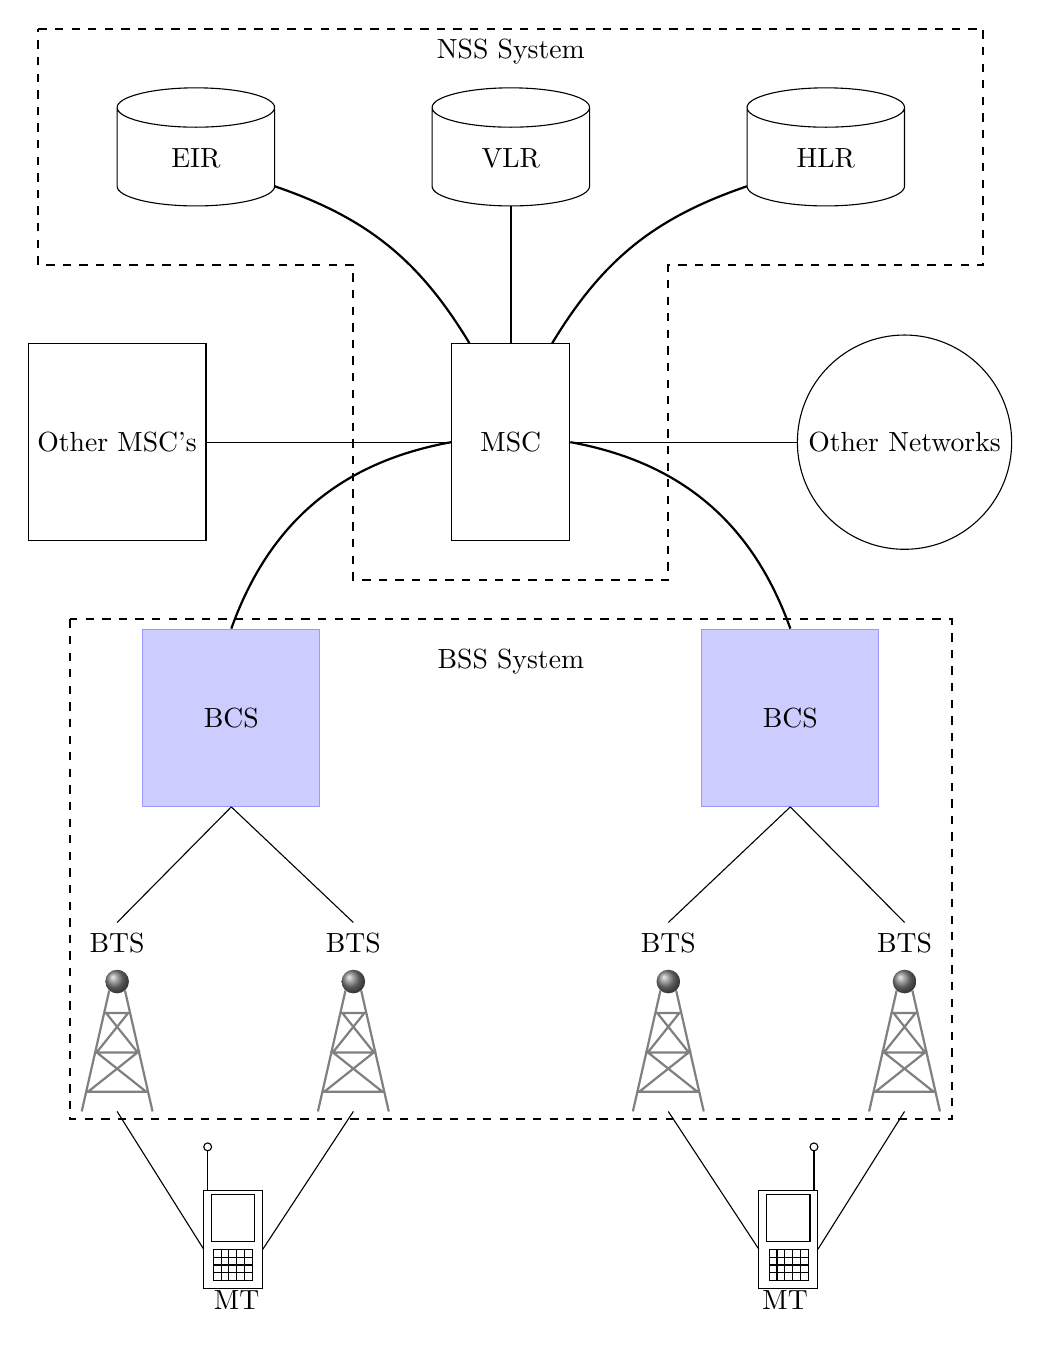
\begin{tikzpicture}[scale=1.0]
		%\draw[step=0.25cm,thin,color=gray] (-6,-8) grid (6,8);
		%drawing of handsets
		%left handset
		\draw (-3.85,-6.20) circle (0.05cm);
		\draw (-3.85,-6.75) -- (-3.85,-6.25);
		\draw (-3.9,-8) node [below=0.15cm,right=0.005cm] {MT} rectangle (-3.15,-6.75);
		\draw (-3.8,-7.4) rectangle (-3.25,-6.8);
		\foreach \x in {0.0,0.1,0.2,0.3,0.4}
		{
			\foreach \y in {0.0,0.1,0.2,0.3}
			{
				\draw (-3.78 + \x,-7.6 - \y) rectangle (-3.68 + \x,-7.5 - \y);
			}
		}
		%right handset
		\draw (3.85,-6.20) circle (0.05cm);
		\draw (3.85,-6.75) -- (3.85,-6.25);
		\draw (3.9,-8) node [below=0.15cm,left=0.005cm] {MT} rectangle (3.15,-6.75);
		\draw (3.8,-7.4) rectangle (3.25,-6.8);
		\foreach \x in {0.0,0.1,0.2,0.3,0.4}
		{
			\foreach \y in {0.0,0.1,0.2,0.3}
			{
				\draw (3.38 + \x,-7.6 - \y) rectangle (3.28 + \x,-7.5 - \y);
			}
		}
		%Drawing of the BTS's
		\begin{scope}
			\foreach \x in {-5,-2,2,5}
			{
				\path (\x,-4.1) coordinate (TowerCirlce);
				\path (\x - 0.10,-4.215) coordinate (startLeftMast);
				\path (\x + 0.10,-4.215) coordinate (startRightMast);
				\path (\x - 0.45,-5.75) coordinate (endLeftMast);
				\path (\x + 0.45,-5.75) coordinate (endRightMast);
				\path (\x - 0.140,-4.5) coordinate (startTopHorizontalBar);
				\path (\x + 0.140,-4.5) coordinate (endTopHorizontalBar);
				\path (\x - 0.260,-5) coordinate (startMiddelHorizontalBar);
				\path (\x + 0.260,-5) coordinate (endMiddelHorizontalBar);
				\path (\x - 0.370,-5.5) coordinate (startBottomHorizontalBar);
				\path (\x + 0.370,-5.5) coordinate (endBottomHorizontalBar);
						\draw [thick,color=gray] (startLeftMast) -- (endLeftMast) (startRightMast) -- (endRightMast) (startMiddelHorizontalBar) -- (endTopHorizontalBar) -- (startTopHorizontalBar) -- (endMiddelHorizontalBar) -- (startMiddelHorizontalBar) -- (endBottomHorizontalBar) -- (startBottomHorizontalBar) -- (endMiddelHorizontalBar) -- cycle;
					\shade [ball color=gray] (TowerCirlce) circle (0.15) node [above=0.25cm] {BTS};
			}
		\end{scope}
		%Lines connecting Handsets with BTS's
		%Left
		\draw (-5,-5.75) -- (-3.9,-7.5);
		\draw (-2,-5.75) -- (-3.15,-7.5);
		%Right
		\draw (5,-5.75) -- (3.9,-7.5);
		\draw (2,-5.75) -- (3.15,-7.5);
		%Drawing of BCS's
		\begin{scope}
			\node (LeftBCS) at (-3.55,-0.75) [shape=rectangle,draw=blue!40, fill=blue!20,minimum size = 2.25cm] {BCS};
			\draw (LeftBCS.south) -- (-5,-3.35);
			\draw (LeftBCS.south) -- (-2,-3.35);
			\node (RightBCS) at (3.55,-0.75) [shape=rectangle,draw=blue!40, fill=blue!20,minimum size = 2.25cm] {BCS};
			\draw (RightBCS.south) -- (5,-3.35);
			\draw (RightBCS.south) -- (2,-3.35);
			\draw [dashed,thick,color=black] (-5.6,0.5) rectangle (5.6,-5.85) (0,0.25) node [anchor=north] {BSS System};
		\end{scope}
		%Draw MSC
		\node (MiddelMSC) at (0,2.75) [shape=rectangle,draw=black,minimum height=2.5cm, minimum width=1.5cm] {MSC};
		\draw [thick] (MiddelMSC.west) to [bend right=30] (LeftBCS.north);
		\draw [thick] (MiddelMSC.east) to [bend left=30] (RightBCS.north);
		\node (LeftMSC) at (-5,2.75) [shape=rectangle,draw=black,minimum height=2.5cm, minimum width=1.5cm] {Other MSC's};
		\node (OtherNetworks) at (5,2.75) [shape=circle,draw=black] {Other Networks};
		\draw (LeftMSC.east) to (MiddelMSC);
		\draw (MiddelMSC) to (OtherNetworks);
		%Databases
		\draw (0,7) circle (1cm and .25cm) node [below=0.40cm] {VLR} ++ (-1,-1) arc (180:360:1cm and .25cm) ++ (-2.0,1) -- (-1.0,6) ++ (2.0,1) -- (1.0,6);
		\draw (-4,7) circle (1cm and .25cm) node [below=0.40cm] {EIR} ++ (-1,-1) arc (180:360:1cm and .25cm) ++ (-2.0,1) -- (-5.0,6) ++ (2.0,1) -- (-3.0,6);
		\draw (4,7) circle (1cm and .25cm) node [below=0.40cm] {HLR} ++ (-1,-1) arc (180:360:1cm and .25cm) ++ (-2.0,1) -- (3.0,6) ++ (2.0,1) -- (5.0,6);
		\draw[thick] (-3,6) to [bend left=20] (MiddelMSC);
		\draw[thick] (0,5.75) to (MiddelMSC);
		\draw[thick] (3,6) to [bend right=20] (MiddelMSC);
		\draw[dashed,thick,color=black] (-6,8) -- (0,8) node [anchor=north] {NSS System} -- (6,8) -- (6,5) -- (2,5) -- (2,1) -- (-2,1) -- (-2,5) -- (-6,5) -- (-6,8) -- cycle;
	\end{tikzpicture}
\end{document}
